\documentclass[11pt]{article}
\usepackage[margin=0.7in]{geometry}
\usepackage{graphicx} %figures
\usepackage{titling}
\usepackage{color}
\usepackage{comment}
\usepackage[none]{hyphenat} %surround text in {} to prevent hyphenation
\usepackage{multirow} %helps tables
\usepackage{array} %helps tables
\usepackage{url}
\usepackage{enumitem}
\usepackage{bold-extra} %allows using small caps and bold series in the same time (use case)

%squeezed itemize for table.
\newenvironment{packed_itemize}{
\begin{itemize}
 % \setlength{}{0pt}
  \setlength{\itemsep}{1pt}
  \setlength{\parskip}{0pt}
  \setlength{\parsep}{0pt}
}{\end{itemize}}



\newenvironment{usecase}{%
	%\def\title$$1{  {\Large\bf{Use Case} ##1} \\}
	\def\title##1{ {\large \bfseries  \scshape {Use Case:} ##1} \\ }
 	\def\id##1{{\bf Indentifier} ##1\\}
	\def\des##1{ {\bf Description:} ##1\\}
	\def\actors##1{ {\bf Actors:} ##1\\}
    	\def\pre##1{ {\bf Preconditions:} ##1 \\} %
    	\def\flow##1{ {\bf Flow of Events} ##1}%
    	\renewenvironment{enumerate}{%
        	\begin{itemize}[nolistsep]\small}%
        	{\end{itemize}}
	\def\post##1{ {\bf Preconditions:} ##1 \\}
}{\vspace{.05in}}

\title{YAExs Elaboration}
\author{TimeFinders: Andrew Karnani, Auston Sterling, Jeffrey Rodowicz and Vera Axelrod}
\date{October 11, 2012}

\begin{document}
\maketitle
\tableofcontents
\vspace{0.2in}
\hrule
\vspace{1in}


%%%%%%%%%%%%%%%%%%%%%%%%%%%%%%%%%%%%%%%%%%%
%%%%%%%%%%%%%%%%%%%%%%%%%%%%%%%%%%%%%%%%%%%
\section{Domain Model}
%Our domain model diagram is shown in Figure \ref{fig:Domain}.

% To include the figure just save the Domain Model diagram in the same directory
% as this tex file, then change {DomainModel.png} to the filename.
% Reference this figure in the text as \ref{fig:Domain}
\begin{comment}
\begin{figure}
	\centering
		\includegraphics[width = \textwidth]{DomainModel.png}
	\caption{Domain Model}
	\label{fig:Domain}
\end{figure}
\end{comment}

%%%%%%%%%%%%%%%%%%%%%%%%%%%%%%%%%%%%%%%%%%%
%%%%%%%%%%%%%%%%%%%%%%%%%%%%%%%%%%%%%%%%%%%
\section{Supplemental Specification}


\begin{tabular}{|m{1in}|m{0.3in}|m{0.6in}|m{4.5in}|}
\hline
\textbf{Category}  & \textbf{ID}  & \textbf{Priority}        & \textbf{Description} \\
\hline\hline
%%%%%%%%%%%%%%%%%%%%
\multirow{3}{*}{Functionality }
 & F01 & Must
 & Description \\  \cline{2-4}
%%%%%
 & F02 & Should
 & Description \\  \cline{2-4}
%%%%%
 & F03 & Could
 & Description \\ \hline

%%%%%%%%%%%%%%%%%%%%
\multirow{3}{*}{Usability }
 & F04 & Must
 & Description \\  \cline{2-4}
%%%%%
 & F05 & Should
 & Description \\  \cline{2-4}
%%%%%
 & F06 & Could
 & Description \\ \hline

%%%%%%%%%%%%%%%%%%%%
\multirow{3}{*}{Reliability }
 & F07 & Must
 & Description \\  \cline{2-4}
%%%%%
 & F08 & Should
 & Description \\  \cline{2-4}
%%%%%
 & F09 & Could
 & Description \\ \hline


%%%%%%%%%%%%%%%%%%%%
\multirow{3}{*}{Performance }
 & F07 & Must
 & Description \\  \cline{2-4}
%%%%%
 & F08 & Should
 & Description \\  \cline{2-4}
%%%%%
 & F09 & Could
 & Description \\ \hline

%%%%%%%%%%%%%%%%%%%%
\multirow{3}{*}{Maintainability}
 & F07 & Must
 & Description \\  \cline{2-4}
%%%%%
 & F08 & Should
 & Description \\  \cline{2-4}
%%%%%
 & F09 & Could
 & Description \\ \hline

%%%%%%%%%%%%%%%%%%%%
\multirow{3}{*}{Configurability}
 & F07 & Must
 & Description \\  \cline{2-4}
%%%%%
 & F08 & Should
 & Description \\  \cline{2-4}
%%%%%
 & F09 & Could
 & Description \\ \hline
\end{tabular}

\textcolor{red}{Constraints?}

%%%%%%%%%%%%%%%%%%%%%%%%%%%%%%%%%%%%%%%%%%%
%%%%%%%%%%%%%%%%%%%%%%%%%%%%%%%%%%%%%%%%%%%
\clearpage
\section{Deployment}

%Our deployment diagram is shown in Figure \ref{fig:Deploy}.

% To include the figure just save the Deployment diagram in the same directory
% as this tex file, then change {DeploymentDiagram.png} to the filename,
% and remove the comments.
% Reference this figure in the text as \ref{fig:Deplot}
\begin{figure}[ht]
	\centering
		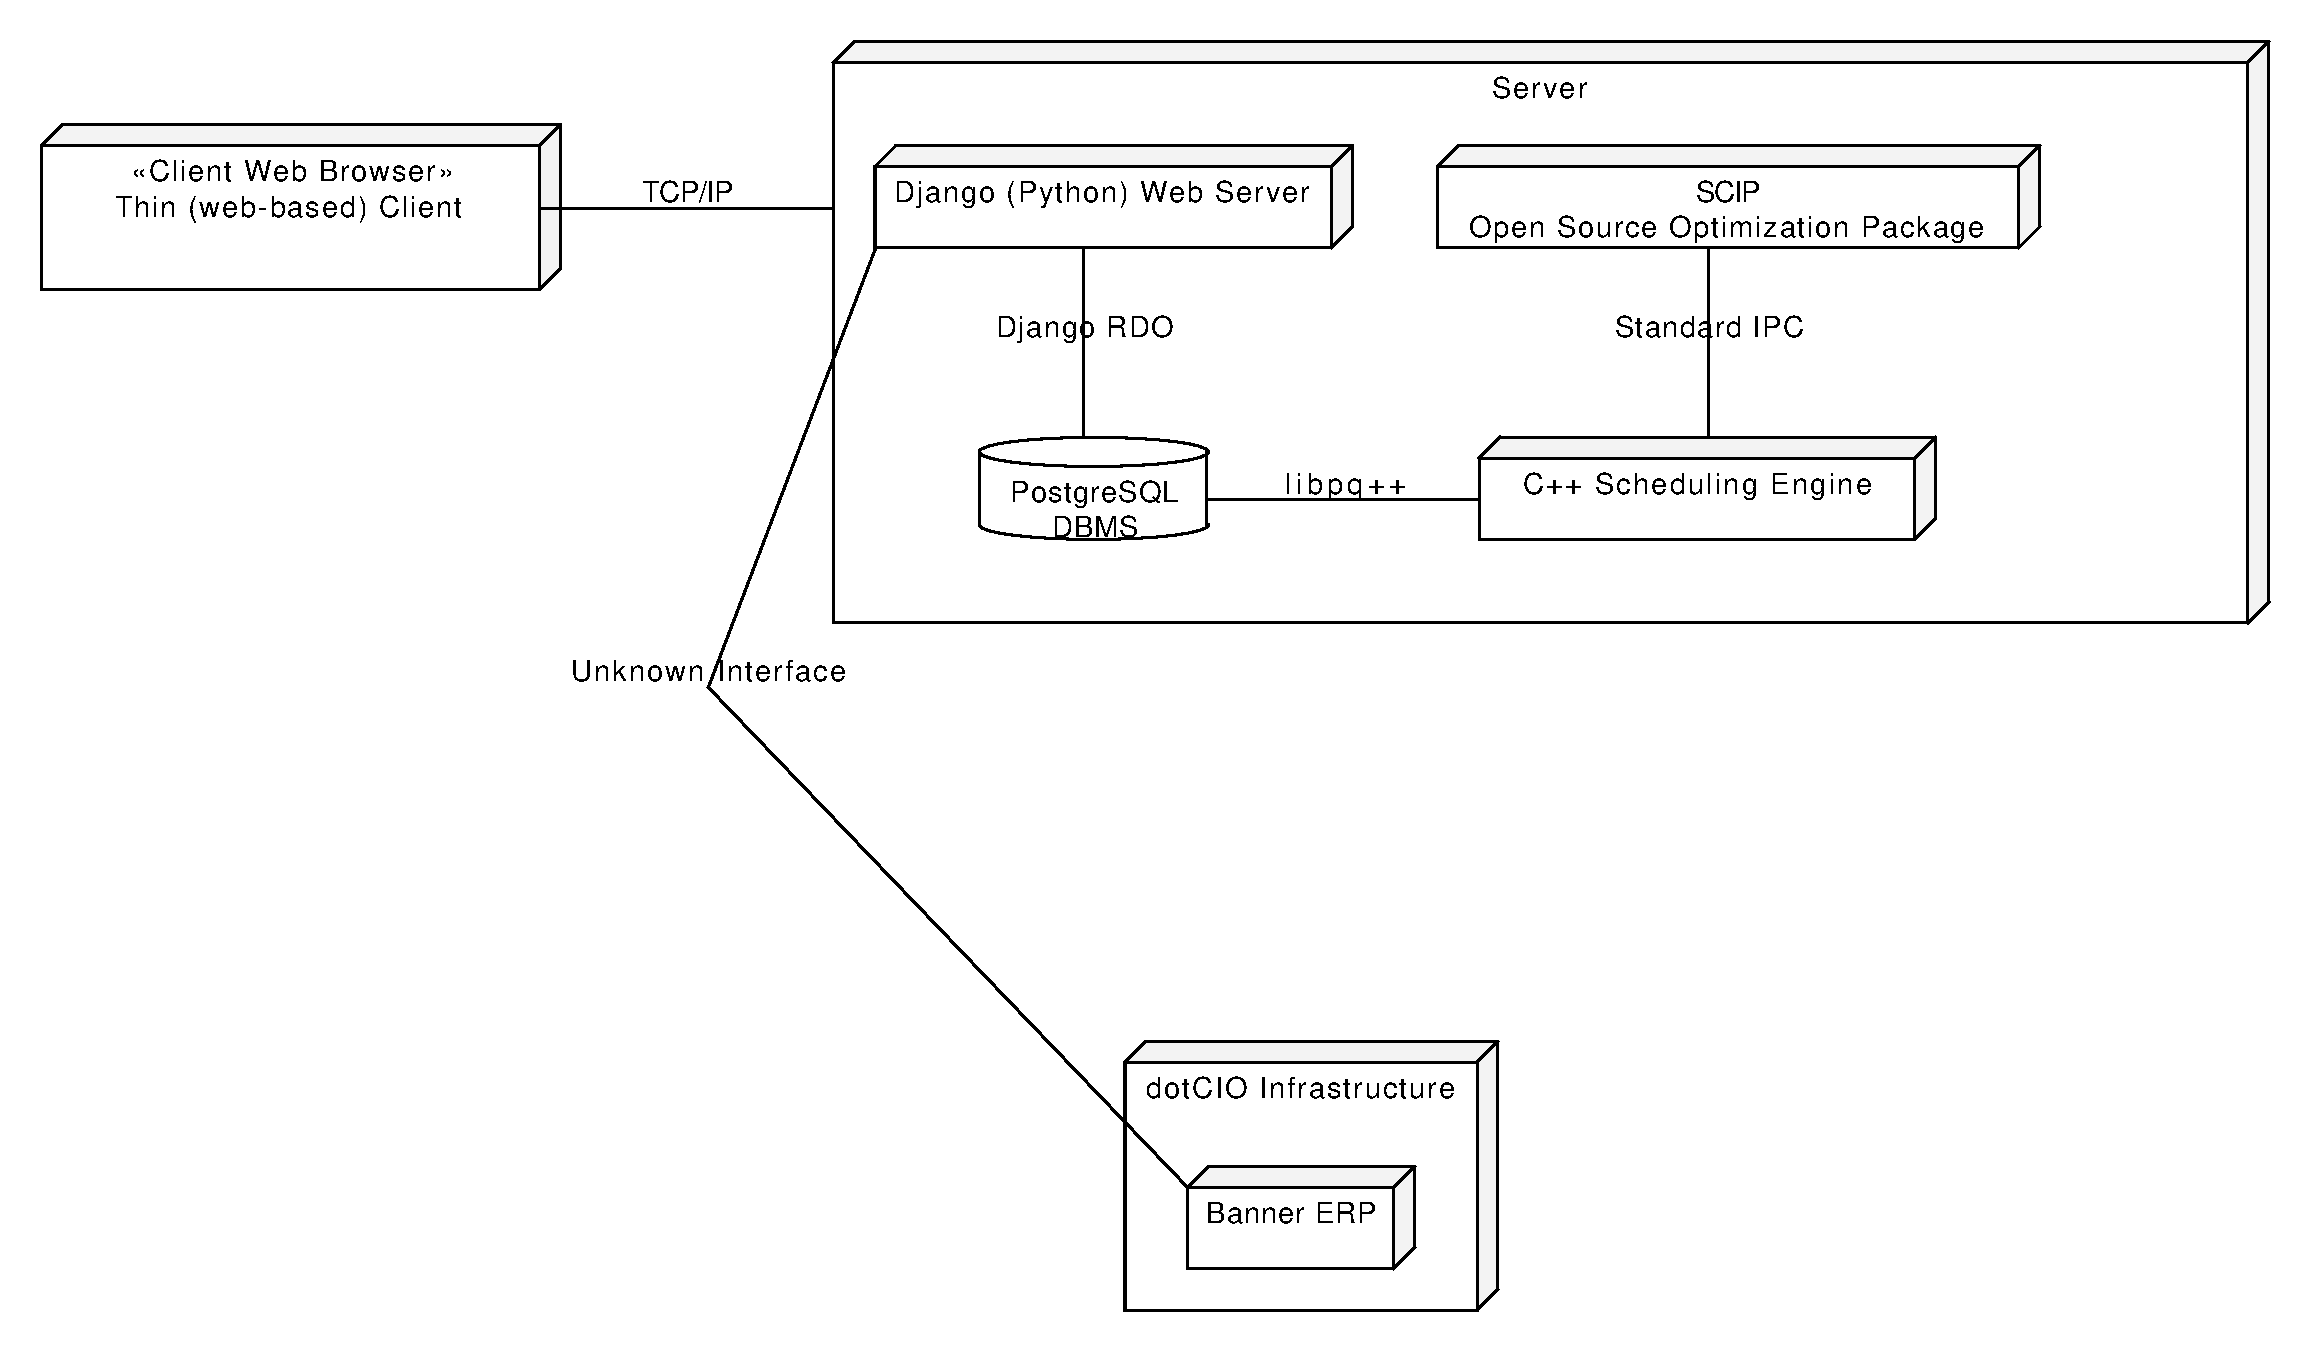
\includegraphics[width = \textwidth]{deploymentdiagram.pdf}
	\caption{Deployment Diagram}
	\label{fig:Deploy}
\end{figure}


%%%%%%%%%%%%%%%%%%%%%%%%%%%%%%%%%%%%%%%%%%%
%%%%%%%%%%%%%%%%%%%%%%%%%%%%%%%%%%%%%%%%%%%
\section{Use Cases}


        \begin{usecase}
	\title{Logging in}
	  \id{S01}
	\des{This is a test use case}
	\actors{Some actors}
	\pre{preconditions!}
	\flow{}
            \begin{enumerate}
                \item User navigates to the YAExS website
                \item User is prompted for RCS ID and password
		\item If the login information is correct:
			\begin{itemize}
				\item If the user is in the Registrar's office: Show the Regisrar main menu.
				\item If the user is a department scheduler: show the department scheduler main page
				\item Else: Display a warning message and prompt for input again.
		\item Else, login information incorrect. Display a warning message and prompt for input agatin
			\end{itemize}
            \end{enumerate}
	\post{The user is logged in and switched to the main page.}
        \end{usecase}

%%%%%%%%%%%%%%%%%%%%%%%%%%%%%%%%%%%%%%%%%%%
%%%%%%%%%%%%%%%%%%%%%%%%%%%%%%%%%%%%%%%%%%%
\section{Work Breakdown}




%%%%%%%%%%%%%%%%%%%%%%%%%%%%%%%%%%%%%%%%%%%
%%%%%%%%%%%%%%%%%%%%%%%%%%%%%%%%%%%%%%%%%%%
\section{Project Schedule}  %Vera


\textcolor{red}{HERE IS THE OLD SCHEDULE}

\begin{tabular}{|m{0.9in}|m{0.9in}|m{4in}|m{.8in}|}
\hline
\textbf{Phases}  & \textbf{Iterations}  & \textbf{Tasks}        & \textbf{Milestones} \\
\hline\hline
%%%%%%%%%%%%%%%%%%%%
Inception 09/06 - 09/24 &
Iteration I 09/06 - 09/24 & \vspace{0.1in}
Inception Deliverables:
	 \begin{packed_itemize}
	\vspace{-0.15in}
		\item Vision Statement
		\item Use Scenarios
		\item Project Schedule
	\vspace{-0.15in}
	\end{packed_itemize}
	& Inception Complete\\
\hline
%%%%%%%%%%%%%%%%%%%%
Elaboration 09/24-10/11&
Iteration II 09/24 - 10/01&  \vspace{0.1in}
Elaboration Deliverables:
	 \begin{packed_itemize}
	\vspace{-0.15in}
		\item Domain Model Diagram
		\item Supplemental Specification
		\item Deployment Diagram
		\item Use Cases
		\item Work Breakdown Structure
		\item Updated Project Schedule
   \end{packed_itemize}

\raggedright{
Instructor and Registrar User Interface Prototype
}

Collect Sample Data from Registrar
& Elaboration Complete
\\
\hline

%%%%%%%%%%%%%%%%%%%%
\multirow{10}{*}{Construction }
 &
 Iteration III 10/01 - 10/12 & \vspace{0.1in}
 Design of System:
	\begin{packed_itemize}
		\vspace{-0.15in}
		\item Static Class Diagram
		\item Design Approach
		\item Select the Optimization Software
	\end{packed_itemize}

 Design of Functions:
	\begin{packed_itemize}
		\vspace{-0.15in}
		\item Sequence Diagram
		\item  Design Pattern
	\end{packed_itemize}

 Implementation \# 1
	\begin{packed_itemize}
	\vspace{-0.15in}
		\item Code and Database Skeleton
		\item Major Classes
	\vspace{-0.15in}
	\end{packed_itemize}
 & Design Complete \\  \cline{2-4}
%%%%%
&
 Iteration IV 10/12 - 10/29 & \vspace{0.1in}
 Implementation \# 2:
\emph{Must} features:
	\begin{packed_itemize}
	\vspace{-0.15in}
		\item Cross-reference course detection
		\item Schedule exams and assign rooms
		\item Interface to display exam schedule
	\end{packed_itemize}

{\raggedright
Sprint \# 1 Deliverable:
Object Calisthenics Sample Code }
 & Iterative Release \\  \cline{2-4}
%%%%%
 &
 Iteration IV 10/29 - 11/19 & \vspace{0.1in}
 Implementation \# 3: Additional Features
	\begin{packed_itemize}
	\vspace{-0.15in}
		\item Instructor exam sign-up website
		\item Registrar exam schedule creation website
		\item Warm start the exam scheduling process
	\end{packed_itemize}

Sprint \# 2 Deliverables:
 Testing Documents, Code Review &
Stakeholder Review \#1
and
Beta Release \\ \hline
%%%%%%%%%%%%%%%%%%%%
Transition  11/19 - 12/06 &
Iteration V 11/19 - 12/06 & \vspace{0.1in}
Implementation \#4:
	\begin{packed_itemize}
		\vspace{-0.15in}
		\item Coordination of features
		\item Integrate entire system
	\end{packed_itemize}
Final Test Results

Final Deliverables:
	\begin{packed_itemize}
	\vspace{-0.15in}
		\item Evidence of Best Practices
		\item Peer Reviews
	\vspace{-0.15in}
	\end{packed_itemize}
&
Stakeholder Review 2 and Final Release \\
\hline
\end{tabular}


%%%%%%%%%%%%%%%%%%%%%%%%%%%%%%%%%%%%%%%%%%%
%%%%%%%%%%%%%%%%%%%%%%%%%%%%%%%%%%%%%%%%%%%
\section{Contribution Summary}

\begin{tabular}{|m{1.4in}|m{4in}|}
\hline
\textbf{\large Name}     & \textbf{\large Contributions} \\
\hline\hline
%%%%%%%%%%%%%%%%%%%%
 Andrew Karnani
	&
	 \begin{packed_itemize}
		\item
	\end{packed_itemize}
\\
\hline
 Auston Sterling
	&
	 \begin{packed_itemize}
	        \item
	\end{packed_itemize}
\\
\hline
Jeffrey Rodowicz
	&
	 \begin{packed_itemize}
		\item
	\end{packed_itemize}
\\
\hline
Vera Axelrod
	&
	 \begin{packed_itemize}
		\item
	\end{packed_itemize}
\\
\hline
\end{tabular}

%%%%%%%%%%%%%%%%%%%%%%%%%%%%%%%%%%%%%%%%%%%
%%%%%%%%%%%%%%%%%%%%%%%%%%%%%%%%%%%%%%%%%%%
\section{Status Report}

\subsection{Things We've Done}
\begin{itemize}
\item
\end{itemize}

\subsection{Challenges}
\begin{itemize}
\item
\end{itemize}

\subsection{Upcoming Plans}
\begin{itemize}
\item
\end{itemize}
\end{document}
